\section{Einführung in die Programmierung}

\begin{frame}{Erwartungen und Vorkenntnisse}
    \begin{itemize}
        \item Erwartungen an den Kurs?
        \item Bereits Programmierkenntnisse aus Schule/Universität?
        \item Kursziele 
            \begin{itemize}
                \item grundlegendes Verständnis
                \item ``mit Informatikern reden können"
                \item Angst nehmen
            \end{itemize}
    \end{itemize}
\end{frame}

\begin{frame}[fragile]{Die Programmiersprache Python}
\begin{columns}
    \column{0.5\textwidth}
    \begin{itemize}
        \item Warum Python?
            \begin{itemize}
                \item flache Lernkurve, sehenswerte Ergebnisse bereits nach dem ersten Tag
                \item verankert in Forschung und Wirtschaft
                \item der englischen Sprache sehr änhlich
                \newline
                \newline
                \newline
                \newline
                \newline
\begin{lstlisting}[basicstyle=\tiny, frame=none]
languages = ["C", "C++", "Java", "Python", "Fortran"]
modern_languages = list( (x for x in languages if x is not "Fortran") )
\end{lstlisting}
           \end{itemize}

    \end{itemize}
    \column{0.5\textwidth}
    \centering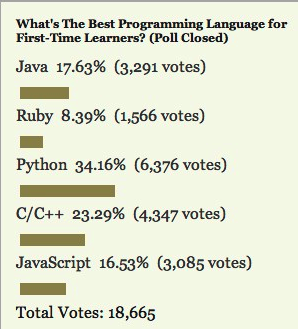
\includegraphics[scale=0.5]{images/best_lang} 
\end{columns}
\end{frame}

